\documentclass[woside,a4paper,12pt]{article}\usepackage[]{graphicx}\usepackage[]{color}
%% maxwidth is the original width if it is less than linewidth
%% otherwise use linewidth (to make sure the graphics do not exceed the margin)
\makeatletter
\def\maxwidth{ %
  \ifdim\Gin@nat@width>\linewidth
    \linewidth
  \else
    \Gin@nat@width
  \fi
}
\makeatother

\definecolor{fgcolor}{rgb}{0.345, 0.345, 0.345}
\newcommand{\hlnum}[1]{\textcolor[rgb]{0.686,0.059,0.569}{#1}}%
\newcommand{\hlstr}[1]{\textcolor[rgb]{0.192,0.494,0.8}{#1}}%
\newcommand{\hlcom}[1]{\textcolor[rgb]{0.678,0.584,0.686}{\textit{#1}}}%
\newcommand{\hlopt}[1]{\textcolor[rgb]{0,0,0}{#1}}%
\newcommand{\hlstd}[1]{\textcolor[rgb]{0.345,0.345,0.345}{#1}}%
\newcommand{\hlkwa}[1]{\textcolor[rgb]{0.161,0.373,0.58}{\textbf{#1}}}%
\newcommand{\hlkwb}[1]{\textcolor[rgb]{0.69,0.353,0.396}{#1}}%
\newcommand{\hlkwc}[1]{\textcolor[rgb]{0.333,0.667,0.333}{#1}}%
\newcommand{\hlkwd}[1]{\textcolor[rgb]{0.737,0.353,0.396}{\textbf{#1}}}%
\let\hlipl\hlkwb

\usepackage{framed}
\makeatletter
\newenvironment{kframe}{%
 \def\at@end@of@kframe{}%
 \ifinner\ifhmode%
  \def\at@end@of@kframe{\end{minipage}}%
  \begin{minipage}{\columnwidth}%
 \fi\fi%
 \def\FrameCommand##1{\hskip\@totalleftmargin \hskip-\fboxsep
 \colorbox{shadecolor}{##1}\hskip-\fboxsep
     % There is no \\@totalrightmargin, so:
     \hskip-\linewidth \hskip-\@totalleftmargin \hskip\columnwidth}%
 \MakeFramed {\advance\hsize-\width
   \@totalleftmargin\z@ \linewidth\hsize
   \@setminipage}}%
 {\par\unskip\endMakeFramed%
 \at@end@of@kframe}
\makeatother

\definecolor{shadecolor}{rgb}{.97, .97, .97}
\definecolor{messagecolor}{rgb}{0, 0, 0}
\definecolor{warningcolor}{rgb}{1, 0, 1}
\definecolor{errorcolor}{rgb}{1, 0, 0}
\newenvironment{knitrout}{}{} % an empty environment to be redefined in TeX

\usepackage{alltt}
\usepackage[sc]{mathpazo}
\usepackage[german]{babel}
\usepackage[utf8]{inputenc}
\usepackage[T1]{fontenc}
\usepackage{float}
\usepackage{graphicx}
\usepackage{subcaption}
\usepackage{geometry}
\geometry{verbose,tmargin=2.5cm,bmargin=2.5cm,lmargin=2.5cm,rmargin=2.5cm}
\setcounter{secnumdepth}{2}
\setcounter{tocdepth}{2}
\usepackage{url}
\usepackage[unicode=true,pdfusetitle,
 bookmarks=true,bookmarksnumbered=true,bookmarksopen=true,bookmarksopenlevel=2,
 breaklinks=false,pdfborder={0 0 1},backref=false,colorlinks=false]
 {hyperref}
\hypersetup{pdfstartview={XYZ null null 1}}
\usepackage{breakurl}
\usepackage{booktabs}
\usepackage{longtable}
\usepackage{array}
\usepackage{multirow}
\usepackage[table]{xcolor}
\usepackage{wrapfig}
\usepackage{float}
\usepackage{colortbl}
\usepackage{pdflscape}
\usepackage{tabu}
\usepackage{threeparttable}
\usepackage{fullpage}
\usepackage{pdflscape}
\IfFileExists{upquote.sty}{\usepackage{upquote}}{}
\begin{document}



\title{somaticGermline TCRBOA6 VCRome - Report}

\author{Patrick Metzger}

\maketitle
\tableofcontents
\clearpage

\section{Qualität der Genomsequenzierung}
\subsection{Raw Quality}

\begin{figure}[H]
  \centering
    \begin{subfigure}[b]{0.45\textwidth}
      \includegraphics[width=\textwidth]{../WES/TCRBOA6-N-WEX.read1_fastqc/Images/per_base_quality.png}
      \caption{Tumor Qualität}
      \label{fig:1}
    \end{subfigure}
    \begin{subfigure}[b]{0.45\textwidth}
      \includegraphics[width=\textwidth]{../WES/TCRBOA6-T-WEX.read1_fastqc/Images/per_base_quality.png}
      \caption{Keimbahn Qualität}
      \label{fig:2}
    \end{subfigure}
\end{figure}

\subsection{Base Quality Score Recalibration (BQSR)}

\begin{figure}[H]
  \centering
    \begin{subfigure}[b]{0.45\textwidth}
      \includegraphics[width=\textwidth]{../WES/somaticGermline_TCRBOA6_VCRome_TD_output.sort.filtered.rmdup.realigned.fixed.recal_fastqc/Images/per_base_quality.png}
      \caption{Tumor Qualität nach BQSR}
      \label{fig:3}
    \end{subfigure}
    \begin{subfigure}[b]{0.45\textwidth}
      \includegraphics[width=\textwidth]{../WES/somaticGermline_TCRBOA6_VCRome_GD_output.sort.filtered.rmdup.realigned.fixed.recal_fastqc/Images/per_base_quality.png}
      \caption{Keimbahn Qualität nach BQSR}
      \label{fig:4}
    \end{subfigure}
\end{figure}

\subsection{Zusammenfassung}

\begin{itemize}
\item VCRome
\item Paired end 100bp
\item TD: 110 Mio. Reads
\item GD: 105 Mio. Reads
\item Gute Qualität der Reads
\end{itemize}

\section{Coverage}

\begin{figure}[H]
\centering
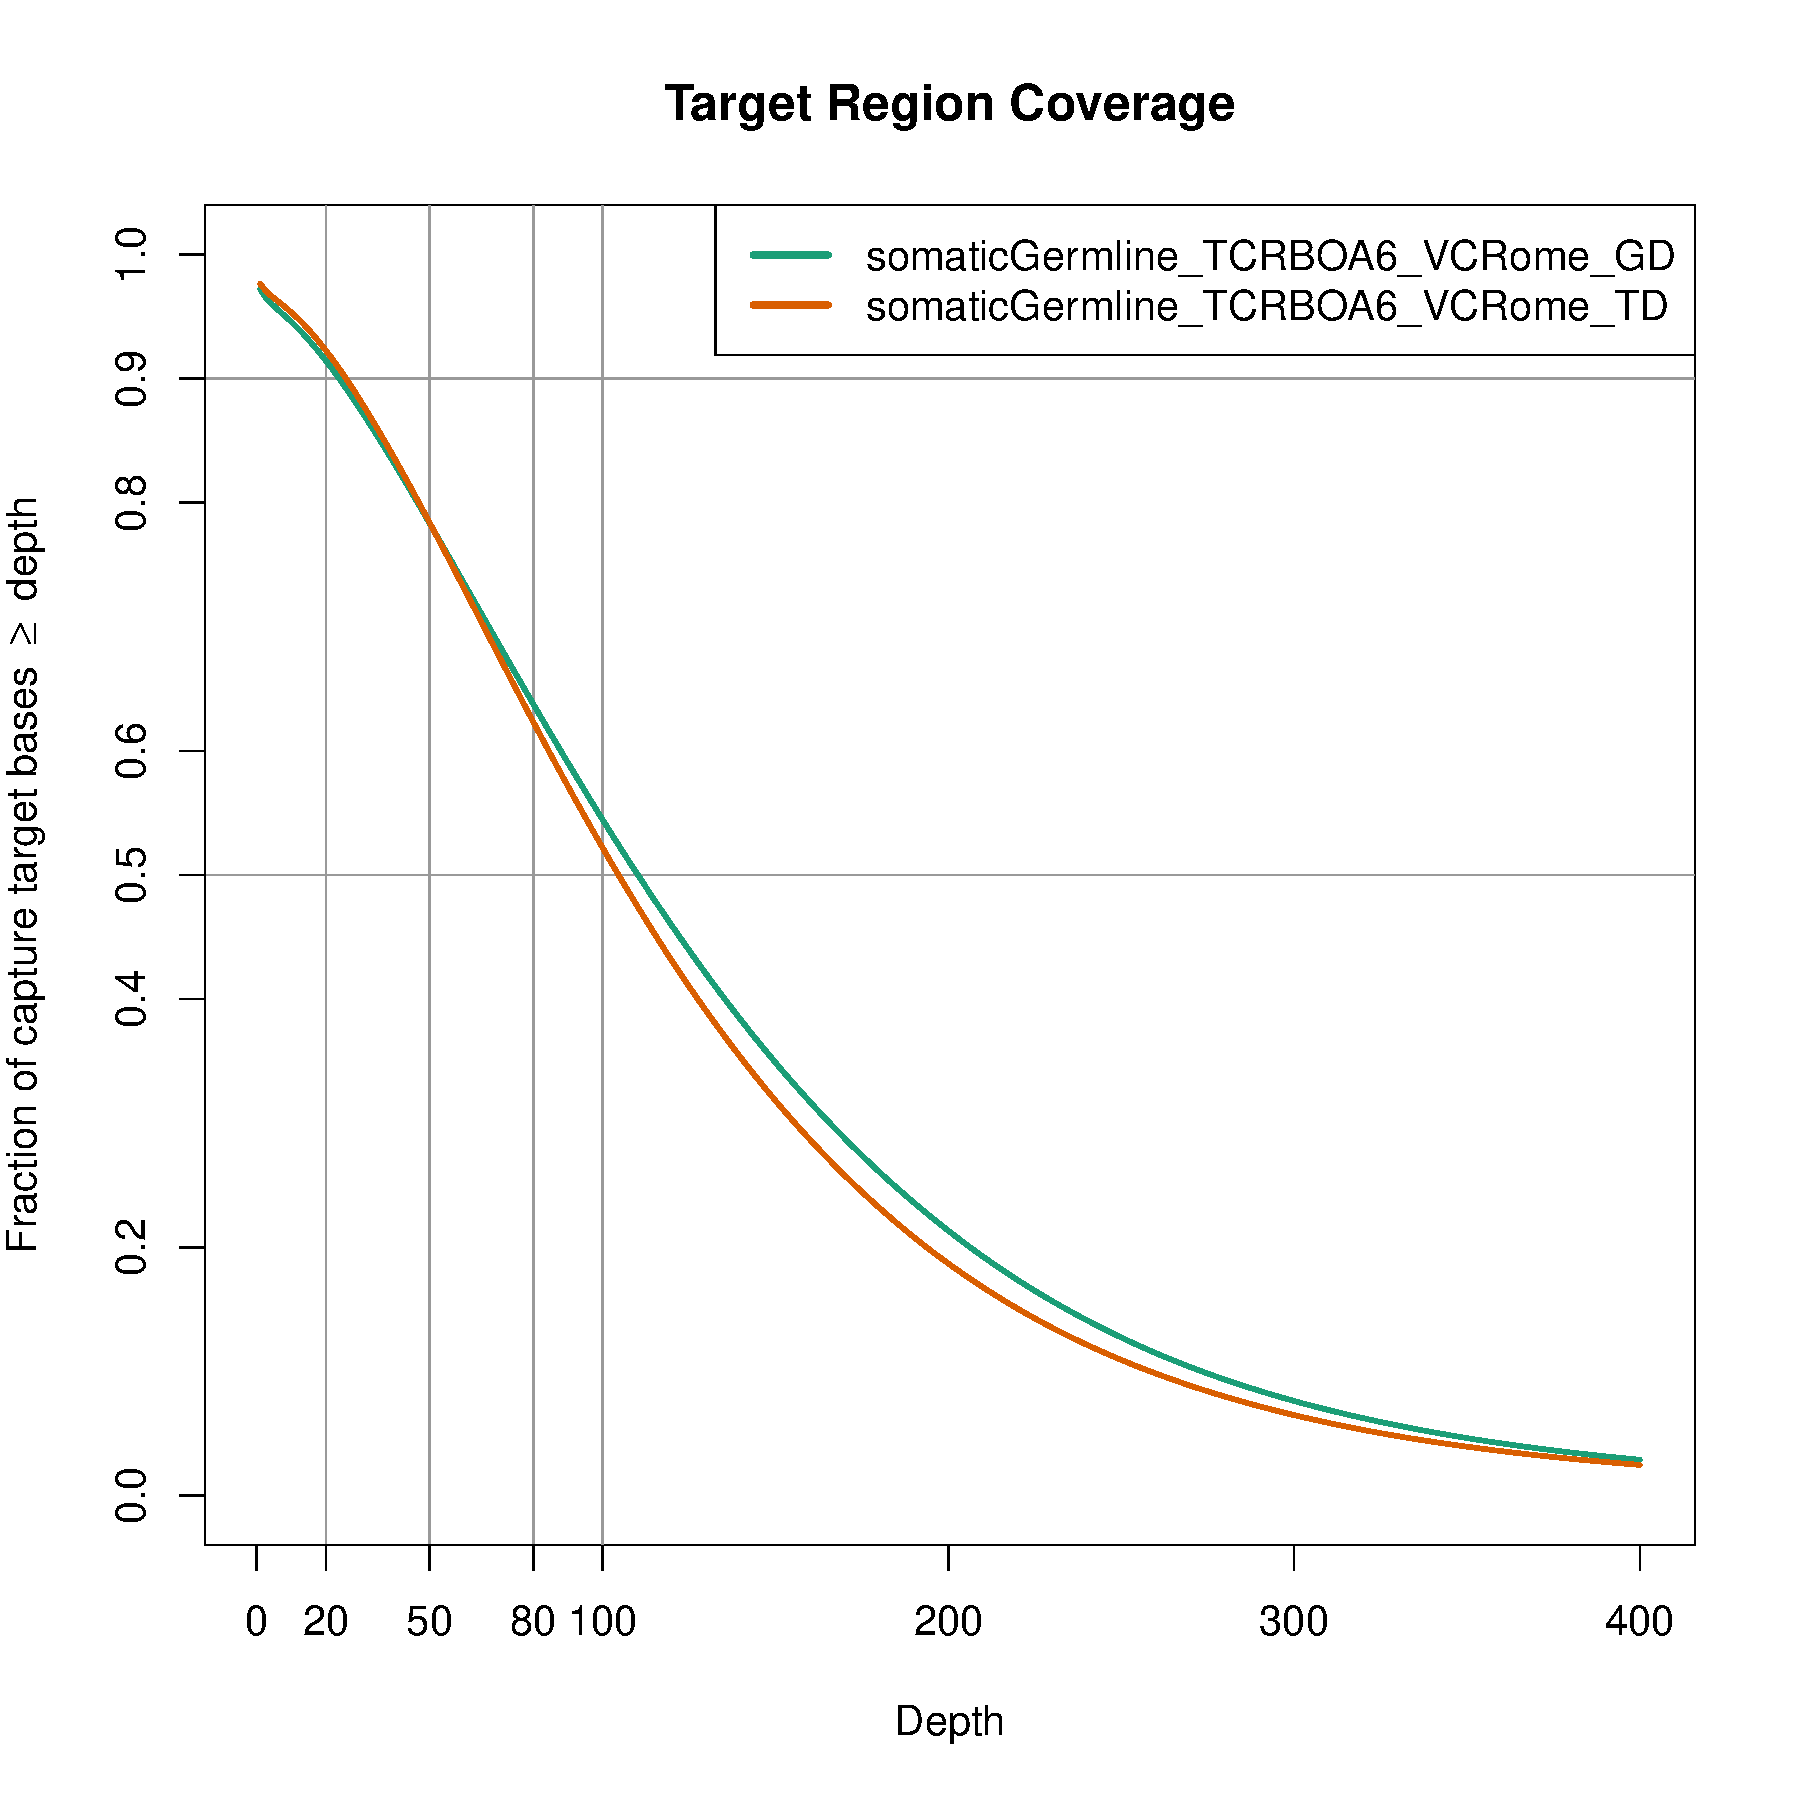
\includegraphics[width=\textwidth]{somaticGermline_TCRBOA6_VCRome_coverage_2019-02-08.pdf}
\caption{Coverage}
\label{fig:5}
\end{figure}

\subsection{Mean Coverage}
\begin{knitrout}
\definecolor{shadecolor}{rgb}{0.969, 0.969, 0.969}\color{fgcolor}\begin{kframe}
\begin{verbatim}
## [1] "Mean Coverage somaticGermline_TCRBOA6_VCRome_GD : 135.2431552"
## [1] "Mean Coverage somaticGermline_TCRBOA6_VCRome_TD : 128.9476502"
\end{verbatim}
\end{kframe}
\end{knitrout}

\clearpage
\section{Mutationsanalyse}
\subsection{Informationen zur Analyse}

\begin{itemize}
\item Aligned zum Referenzgenom UCSC hg19
\item Einschlusskriterien der Mutation
  \begin{itemize}
    \item Mindestens 8 Reads pro Base
    \item Seltene Mutationen (Minor-Allele Frequency (MAF) $< 0.001$, basierend auf gnomAD exome, ExAC, ESP6500 und 1000g)
    \item Keine \grqq Black-listed\grqq{} Gene/Sequenzen
    \item Variant Allele Frequency (VAF) $> 10\%$
  \end{itemize}
  \item Analyse der Mutationen
  \begin{itemize}
  \item Annotation bekannter Mutationen (Cosmic, Clinvar, dbSNP)
  \item Ranking der Wichtigkeit (RVIS Score)
  \item Strukturanalyse der mutierten Proteine (Condel, CADD)
  \end{itemize}
\end{itemize}

\subsection{Somatische Mutationen und Loss of Heterozygosity (LoH)}

\begin{figure}[H]
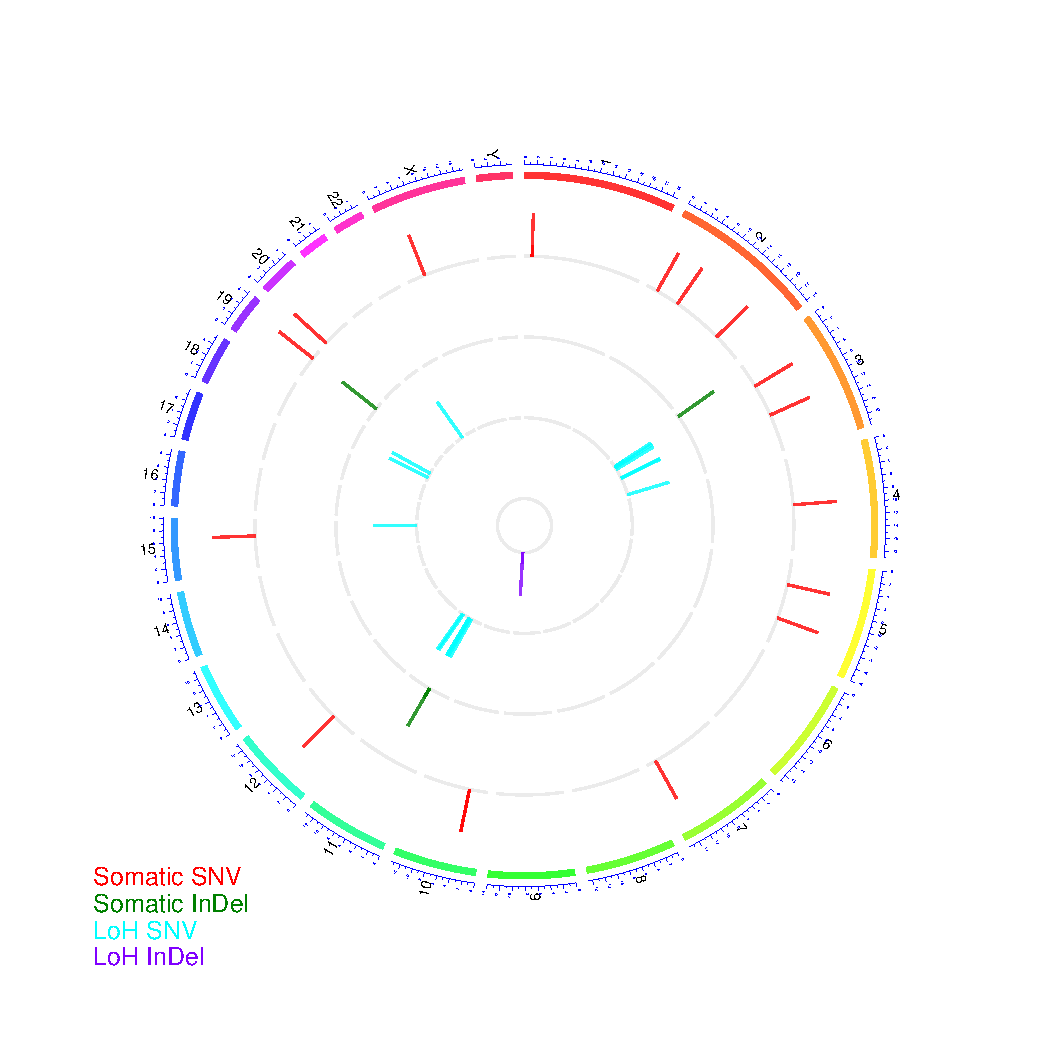
\includegraphics[width=\textwidth]{somaticGermline_TCRBOA6_VCRome_TD_circos_2019-02-08.pdf}
\caption{Circos Plot}
\label{fig:6}
\end{figure}

\clearpage

\begin{knitrout}
\definecolor{shadecolor}{rgb}{0.969, 0.969, 0.969}\color{fgcolor}\rowcolors{2}{gray!6}{white}
\begin{table}[!h]

\caption{\label{tab:unnamed-chunk-2}Zusammenfassung der identifizierten Mutationen}
\centering
\fontsize{12}{14}\selectfont
\begin{tabular}[t]{lrlrrr}
\hiderowcolors
\toprule
Mutationstype & Number of exonic & Zygosity & TS & OG & HS\\
\midrule
\showrowcolors
somatic SNV & 0 & homozygous & 0 & 0 & 0\\
somatic SNV & 17 & heterozygous & 0 & 0 & 0\\
LoH SNV & 16 & - & 0 & 0 & 0\\
somatic InDel & 0 & homozygous & 0 & 0 & 0\\
somatic InDel & 3 & heterozygous & 2 & 0 & 0\\
LoH InDel & 1 & - & 0 & 0 & 0\\
\bottomrule
\end{tabular}
\end{table}
\rowcolors{2}{white}{white}


\end{knitrout}

\begin{itemize}
\item 20 somatische Mutationen (exonisch)
\item 17 Loss of Heterozygosity (LoH)
\item Insgesamt 37 Mutationen
\item Mutationslast 2.37/Mb
\end{itemize}
\begin{knitrout}
\definecolor{shadecolor}{rgb}{0.969, 0.969, 0.969}\color{fgcolor}\begingroup\fontsize{8}{10}\selectfont
\rowcolors{2}{white}{gray!6}

\begin{longtable}[t]{>{\raggedright\arraybackslash}p{5em}>{\raggedright\arraybackslash}p{20em}>{\raggedleft\arraybackslash}p{5em}>{\raggedleft\arraybackslash}p{5em}>{\raggedleft\arraybackslash}p{5em}}
\caption{\label{tab:unnamed-chunk-3}Tumorsuppressoren und Onkogene - Überblick}\\
\hiderowcolors
\toprule
Symbol & Gene Name & TSG & OG & HS\\
\midrule
\showrowcolors
VHL & von Hippel-Lindau tumor suppressor & 1 & 0 & 0\\
MEN1 & menin 1 & 1 & 0 & 0\\
\bottomrule
\end{longtable}
\rowcolors{2}{white}{white}\endgroup{}


\end{knitrout}
\clearpage

\begin{landscape}
\subsection{Tumorsuppressoren und Onkogene}
\thispagestyle{empty}
\begin{knitrout}
\definecolor{shadecolor}{rgb}{0.969, 0.969, 0.969}\color{fgcolor}\rowcolors{2}{gray!6}{white}
\begin{table}[H]

\caption{\label{tab:unnamed-chunk-4}Tumorsuppressoren und Onkogene}
\centering
\fontsize{8}{10}\selectfont
\begin{tabular}[t]{>{\raggedright\arraybackslash}p{2em}>{\raggedright\arraybackslash}p{6em}>{\raggedright\arraybackslash}p{6em}>{\raggedright\arraybackslash}p{6em}>{\raggedright\arraybackslash}p{2em}>{\raggedright\arraybackslash}p{2em}>{\raggedright\arraybackslash}p{2em}>{\raggedleft\arraybackslash}p{2em}>{\raggedleft\arraybackslash}p{2em}>{\raggedleft\arraybackslash}p{6em}>{\raggedright\arraybackslash}p{6em}>{\raggedright\arraybackslash}p{2em}>{\raggedleft\arraybackslash}p{2em}>{\raggedright\arraybackslash}p{2em}>{\raggedright\arraybackslash}p{2em}>{\raggedright\arraybackslash}p{8em}}
\hiderowcolors
\toprule
\rotatebox{45}{Symbol} & \rotatebox{45}{Gene Name} & \rotatebox{45}{Exonic Function} & \rotatebox{45}{Aminoacid Change} & \rotatebox{45}{VAF} & \rotatebox{45}{Zygosity} & \rotatebox{45}{Reads} & \rotatebox{45}{TSG} & \rotatebox{45}{OG} & \rotatebox{45}{HS} & \rotatebox{45}{TARGET} & \rotatebox{45}{MAF} & \rotatebox{45}{CADD} & \rotatebox{45}{Condel} & \rotatebox{45}{CLINSIG} & \rotatebox{45}{COSMIC}\\
\midrule
\showrowcolors
VHL & von Hippel-Lindau tumor suppressor & frameshift deletion & p.His125fs & 51\% & het & 51|100 & 1 & 0 & 0 &  & NA & NA & NA & NA & NA\\
MEN1 & menin 1 & frameshift insertion &  & 56.07\% & het & 60|107 & 1 & 0 & 0 &  & NA & NA & NA &  & NA\\
\bottomrule
\end{tabular}
\end{table}
\rowcolors{2}{white}{white}


\end{knitrout}
\clearpage
\subsection{Somatische Mutationen (top20 nach VAF)}
\thispagestyle{empty}
\begin{knitrout}
\definecolor{shadecolor}{rgb}{0.969, 0.969, 0.969}\color{fgcolor}\begingroup\fontsize{8}{10}\selectfont
\rowcolors{2}{white}{gray!6}

\begin{longtable}[t]{>{\raggedright\arraybackslash}p{6em}>{\raggedright\arraybackslash}p{6em}>{\raggedright\arraybackslash}p{6em}>{\raggedright\arraybackslash}p{6em}>{\raggedright\arraybackslash}p{2em}>{\raggedright\arraybackslash}p{2em}>{\raggedright\arraybackslash}p{2em}>{\raggedleft\arraybackslash}p{2em}>{\raggedleft\arraybackslash}p{2em}>{\raggedleft\arraybackslash}p{6em}>{\raggedright\arraybackslash}p{6em}>{\raggedright\arraybackslash}p{2em}>{\raggedleft\arraybackslash}p{2em}>{\raggedright\arraybackslash}p{2em}>{\raggedright\arraybackslash}p{2em}>{\raggedright\arraybackslash}p{8em}}
\caption{\label{tab:unnamed-chunk-5}somatische Mutationen}\\
\hiderowcolors
\toprule
\rotatebox{45}{Symbol} & \rotatebox{45}{Gene Name} & \rotatebox{45}{Exonic Function} & \rotatebox{45}{Aminoacid Change} & \rotatebox{45}{VAF} & \rotatebox{45}{Zygosity} & \rotatebox{45}{Reads} & \rotatebox{45}{TSG} & \rotatebox{45}{OG} & \rotatebox{45}{HS} & \rotatebox{45}{TARGET} & \rotatebox{45}{MAF} & \rotatebox{45}{CADD} & \rotatebox{45}{Condel} & \rotatebox{45}{CLINSIG} & \rotatebox{45}{COSMIC}\\
\midrule
\endfirsthead
\caption[]{somatische Mutationen \textit{(continued)}}\\
\toprule
Symbol & Gene Name & Exonic Function & Aminoacid Change & VAF & Zygosity & Reads & TSG & OG & HS & TARGET & MAF & CADD & Condel & CLINSIG & COSMIC\\
\midrule
\endhead
\
\endfoot
\bottomrule
\endlastfoot
\showrowcolors
GPR156 & G protein-coupled receptor 156 & nonsynonymous SNV & p.Ala608Val & 73.33\% & het & 22|30 & 0 & 0 & 0 & . & NA & 20.900 & N & NA & NA\\
DOCK3 & dedicator of cytokinesis 3 & nonsynonymous SNV & p.Leu1633Phe & 62.16\% & het & 23|37 & 0 & 0 & 0 & . & 0.00e+00 & 19.080 & N & NA & NA\\
MEN1 & menin 1 & frameshift insertion &  & 56.07\% & het & 60|107 & 1 & 0 & 0 &  & NA & NA & NA &  & NA\\
VHL & von Hippel-Lindau tumor suppressor & frameshift deletion & p.His125fs & 51\% & het & 51|100 & 1 & 0 & 0 &  & NA & NA & NA & NA & NA\\
SNX18 & sorting nexin 18 & nonsynonymous SNV & p.Ser613Phe & 40.68\% & het & 24|59 & 0 & 0 & 0 & . & NA & 11.510 & N & NA & NA\\
\addlinespace
PLEKHM2 & pleckstrin homology and RUN domain containing M2 & nonsynonymous SNV & p.Arg830Trp & 40.38\% & het & 126|312 & 0 & 0 & 0 & . & 9.31e-06 & 34.000 & D & NA & ID=COSM6749990, COSM6749991\\
FAM228B & family with sequence similarity 228 member B & unknown & p.Leu316* & 40.35\% & het & 23|57 & 0 & 0 & 0 & . & NA & 35.000 & N & NA & NA\\
NEUROD1 & neuronal differentiation 1 & nonsynonymous SNV & p.Lys39Glu & 40.12\% & het & 67|167 & 0 & 0 & 0 & . & NA & 10.670 & D & NA & NA\\
UNC5C & unc-5 netrin receptor C & nonsynonymous SNV & p.Pro839Ser & 37.41\% & het & 55|147 & 0 & 0 & 0 & . & NA & 23.800 & N & NA & ID=COSM2989103\\
CYBB & cytochrome b-245 beta chain & nonsynonymous SNV & p.Gly512Arg & 35.8\% & het & 63|176 & 0 & 0 & 0 & . & NA & 32.000 & D & NA & NA\\
\addlinespace
ZC3H10 & zinc finger CCCH-type containing 10 & nonsynonymous SNV & p.Val181Asp & 33.94\% & het & 37|109 & 0 & 0 & 0 & . & NA & 9.774 & N & NA & NA\\
CD177 & CD177 molecule & unknown & p.Val240Met & 33.86\% & het & 64|189 & 0 & 0 & 0 & . & NA & 3.844 & NA & NA & NA\\
CEACAM8 & carcinoembryonic antigen related cell adhesion molecule 8 & frameshift deletion & p.Gln16fs & 33.33\% & het & 15|45 & 0 & 0 & 0 & . & NA & NA & NA & NA & NA\\
ATP6V0A4 & ATPase H+ transporting V0 subunit a4 & nonsynonymous SNV & p.Ala706Ser & 32.39\% & het & 23|71 & 0 & 0 & 0 & . & NA & 1.999 & N & NA & NA\\
MEGF10 & multiple EGF like domains 10 & nonsynonymous SNV & p.Ala726Val & 31.5\% & het & 40|127 & 0 & 0 & 0 & . & NA & 24.800 & N & NA & NA\\
\addlinespace
TTC31 & tetratricopeptide repeat domain 31 & nonsynonymous SNV & p.Glu199Gly & 29.55\% & het & 39|132 & 0 & 0 & 0 & . & NA & 23.100 & N & NA & NA\\
ANKRD30A & ankyrin repeat domain 30A & nonsynonymous SNV & p.Cys873Tyr & 28.12\% & het & 9|32 & 0 & 0 & 0 & . & NA & 6.906 & N & NA & NA\\
TMC2 & transmembrane channel like 2 & stopgain & p.Lys165* & 27.88\% & het & 46|165 & 0 & 0 & 0 & . & NA & 37.000 & NA & NA & NA\\
LCTL & lactase like & nonsynonymous SNV & p.Thr36Ile & 26.62\% & het & 37|139 & 0 & 0 & 0 & . & NA & 23.700 & N & NA & NA\\
ANKRD30A & ankyrin repeat domain 30A & nonsynonymous SNV & p.Cys516Tyr & 10.48\% & het & 26|248 & 0 & 0 & 0 & . & NA & 0.001 & N & NA & NA\\*
\end{longtable}
\rowcolors{2}{white}{white}\endgroup{}


\end{knitrout}
\clearpage
\subsection{LoH}
\thispagestyle{empty}
\begin{knitrout}
\definecolor{shadecolor}{rgb}{0.969, 0.969, 0.969}\color{fgcolor}\begingroup\fontsize{8}{10}\selectfont
\rowcolors{2}{white}{gray!6}

\begin{longtable}[t]{>{\raggedright\arraybackslash}p{6em}>{\raggedright\arraybackslash}p{8em}>{\raggedright\arraybackslash}p{6em}>{\raggedright\arraybackslash}p{6em}>{\raggedright\arraybackslash}p{2em}>{\raggedright\arraybackslash}p{2em}>{\raggedright\arraybackslash}p{2em}>{\raggedright\arraybackslash}p{2em}>{\raggedleft\arraybackslash}p{2em}>{\raggedleft\arraybackslash}p{2em}>{\raggedleft\arraybackslash}p{2em}>{\raggedright\arraybackslash}p{6em}>{\raggedright\arraybackslash}p{2em}>{\raggedright\arraybackslash}p{2em}>{\raggedright\arraybackslash}p{2em}>{\raggedright\arraybackslash}p{2em}>{\raggedright\arraybackslash}p{8em}}
\caption{\label{tab:unnamed-chunk-6}LoH}\\
\hiderowcolors
\toprule
\rotatebox{45}{Symbol} & \rotatebox{45}{Gene Name} & \rotatebox{45}{Exonic Function} & \rotatebox{45}{Aminoacid Change} & \rotatebox{45}{VAF\_Normal} & \rotatebox{45}{VAF\_Tumor} & \rotatebox{45}{Reads\_Normal} & \rotatebox{45}{Reads\_Tumor} & \rotatebox{45}{TSG} & \rotatebox{45}{OG} & \rotatebox{45}{HS} & \rotatebox{45}{TARGET} & \rotatebox{45}{MAF} & \rotatebox{45}{CADD} & \rotatebox{45}{Condel} & \rotatebox{45}{CLINSIG} & \rotatebox{45}{COSMIC}\\
\midrule
\showrowcolors
OSBPL10 & oxysterol binding protein like 10 & nonsynonymous SNV & p.Ala437Val & 53.66\% & 78.38\% & 66|124 & 58|74 & 0 & 0 & 0 & . & 8.96e-06 & 33 & D & NA & NA\\
SLC22A13 & solute carrier family 22 member 13 & nonsynonymous SNV & p.Ala77Val & 41.73\% & 76.54\% & 58|139 & 62|81 & 0 & 0 & 0 & . & 8.06e-05 & 3.410 & D & NA & NA\\
ARIH2OS & ariadne RBR E3 ubiquitin protein ligase 2 opposite strand & nonsynonymous SNV & p.Ser166Pro & 51.67\% & 82.05\% & 31|60 & 32|39 & 0 & 0 & 0 & . & 2.70e-05 & 13.20 & N & NA & NA\\
FILIP1L & filamin A interacting protein 1 like & nonsynonymous SNV & p.Lys183Glu & 58.33\% & 85.45\% & 42|72 & 47|55 & 0 & 0 & 0 & . & 8.00e-04 & 10.25 & N & NA & NA\\
NFKBIZ & NFKB inhibitor zeta & nonsynonymous SNV & p.Leu545Pro & 40\% & 77.78\% & 12|30 & 14|18 & 0 & 0 & 0 & . & 9.00e-04 & 27.2 & N & NA & NA\\
\addlinespace
LSG1 & large 60S subunit nuclear export GTPase 1 & nonsynonymous SNV & p.Leu510Phe & 49.23\% & 78.31\% & 64|130 & 65|83 & 0 & 0 & 0 & . & 0.00e+00 & 23.3 & D & NA & NA\\
TNKS1BP1 & tankyrase 1 binding protein 1 & nonsynonymous SNV & p.Arg427Gln & 53\% & 81.03\% & 53|100 & 47|58 & 0 & 0 & 0 & . & 2.00e-04 & 34 & N & NA & ID=COSM1229944\\
LTBP3 & latent transforming growth factor beta binding protein 3 & nonsynonymous SNV & p.Pro488Ser & 51.52\% & 82.09\% & 68|132 & 55|67 & 0 & 0 & 0 & . & NA & 12.94 & D & NA & NA\\
ZNF705E & zinc finger protein 705E & nonsynonymous SNV &  & 42.36\% & 76.61\% & 61|144 & 95|124 & 0 & 0 & 0 & . & NA & NA & NA & NA & NA\\
ZNF705E & zinc finger protein 705E & nonsynonymous SNV &  & 46.31\% & 75\% & 69|149 & 72|96 & 0 & 0 & 0 & . & NA & NA & NA & NA & NA\\
\addlinespace
ALKBH8 & alkB homolog 8, tRNA methyltransferase & nonsynonymous SNV & p.Ser149Cys & 53.33\% & 88.24\% & 24|45 & 45|51 & 0 & 0 & 0 & . & 1.80e-05 & 24.5 & N & NA & NA\\
ANKK1 & ankyrin repeat and kinase domain containing 1 & nonsynonymous SNV & p.Arg295Cys & 51.52\% & 80.49\% & 34|66 & 33|41 & 0 & 0 & 0 & . & 8.96e-06 & 14.80 & N & NA & NA\\
ISG20 & interferon stimulated exonuclease gene 20 & nonsynonymous SNV &  & 55.17\% & 83.05\% & 64|116 & 49|59 & 0 & 0 & 0 & . & NA & NA & NA & NA & NA\\
ZNF521 & zinc finger protein 521 & nonsynonymous SNV & p.Glu484Lys & 57.66\% & 87.83\% & 64|111 & 101|115 & 0 & 0 & 0 & . & 1.80e-05 & 21.9 & N & NA & ID=COSM6830919\\
LIPG & lipase G, endothelial type & nonsynonymous SNV & p.Ser95Arg & 50.91\% & 80.56\% & 28|55 & 29|36 & 0 & 0 & 0 & . & 3.59e-05 & 23.4 & D & NA & NA\\
\addlinespace
BRWD1 & bromodomain and WD repeat domain containing 1 & nonsynonymous SNV & p.Thr1205Ile & 47.5\% & 88.24\% & 19|40 & 30|34 & 0 & 0 & 0 & . & 2.70e-05 & 25.3 & N & NA & NA\\
C9orf147 & chromosome 9 open reading frame 147 & frameshift deletion &  & 66.67\% & 100\% & 6|9 & 16|16 & 0 & 0 & 0 & . & NA & NA & NA & NA & NA\\
\bottomrule
\end{longtable}
\rowcolors{2}{white}{white}\endgroup{}


\end{knitrout}
\end{landscape}

\begin{landscape}
\subsection{Funktionelle Analysen}
\subsubsection{GO}
\thispagestyle{empty}
\begin{knitrout}
\definecolor{shadecolor}{rgb}{0.969, 0.969, 0.969}\color{fgcolor}\rowcolors{2}{gray!6}{white}
\begin{table}[H]

\caption{\label{tab:unnamed-chunk-7}Ergebnisse GO Analyse, top 20}
\centering
\begin{tabular}[t]{lrrll}
\hiderowcolors
\toprule
Term & Count & Size & p-value & adj.P.Val\\
\midrule
\showrowcolors
response to peptide hormone & 3 & 401 & 2.94e-02 & 1e+00\\
response to peptide & 3 & 448 & 3.88e-02 & 1e+00\\
response to abiotic stimulus & 5 & 1153 & 4.06e-02 & 1e+00\\
negative regulation of intracellular signal transduction & 3 & 468 & 4.12e-02 & 1e+00\\
cellular homeostasis & 4 & 822 & 4.55e-02 & 1e+00\\
\addlinespace
neutrophil activation involved in immune response & 3 & 485 & 4.66e-02 & 1e+00\\
neutrophil degranulation & 3 & 485 & 4.66e-02 & 1e+00\\
neutrophil activation & 3 & 490 & 4.78e-02 & 1e+00\\
homeostatic process & 6 & 1621 & 4.84e-02 & 1e+00\\
granulocyte activation & 3 & 495 & 4.90e-02 & 1e+00\\
neutrophil mediated immunity & 3 & 498 & 4.98e-02 & 1e+00\\
\bottomrule
\end{tabular}
\end{table}
\rowcolors{2}{white}{white}


\end{knitrout}
\clearpage
\subsubsection{Consensus}
\thispagestyle{empty}
\begin{knitrout}
\definecolor{shadecolor}{rgb}{0.969, 0.969, 0.969}\color{fgcolor}\rowcolors{2}{gray!6}{white}
\begin{table}[H]

\caption{\label{tab:unnamed-chunk-8}Ergebnisse Consensus Analyse, top 20}
\centering
\fontsize{10}{12}\selectfont
\begin{tabular}[t]{lrrll>{\raggedright\arraybackslash}p{10em}}
\hiderowcolors
\toprule
Term & Count & Size & p-value & adj.P.Val & Symbol\\
\midrule
\showrowcolors
NA & NA & NA & NA & NA & NULL\\
\bottomrule
\end{tabular}
\end{table}
\rowcolors{2}{white}{white}


\end{knitrout}

\clearpage
\subsubsection{Reactome}
\thispagestyle{empty}
\begin{knitrout}
\definecolor{shadecolor}{rgb}{0.969, 0.969, 0.969}\color{fgcolor}\rowcolors{2}{gray!6}{white}
\begin{table}[H]

\caption{\label{tab:unnamed-chunk-9}Ergebnisse Reactome Analyse, top 20}
\centering
\begin{tabular}[t]{lrrll}
\hiderowcolors
\toprule
Term & Count & Size & p-value & adj.P.Val\\
\midrule
\showrowcolors
Immune System & 7 & 2002 & 4.34e-02 & 1e+00\\
Neutrophil degranulation & 3 & 476 & 4.49e-02 & 1e+00\\
\bottomrule
\end{tabular}
\end{table}
\rowcolors{2}{white}{white}


\end{knitrout}
\clearpage
\subsubsection{Hallmarks of Cancer}
\thispagestyle{empty}
\begin{knitrout}
\definecolor{shadecolor}{rgb}{0.969, 0.969, 0.969}\color{fgcolor}\rowcolors{2}{gray!6}{white}
\begin{table}[H]

\caption{\label{tab:unnamed-chunk-10}Ergebnisse Hallmarks Analyse, top 20}
\centering
\begin{tabular}[t]{lrrll}
\hiderowcolors
\toprule
Term & Count & Size & p-value & adj.P.Val\\
\midrule
\showrowcolors
NA & NA & NA & NA & NA\\
\bottomrule
\end{tabular}
\end{table}
\rowcolors{2}{white}{white}


\end{knitrout}
\clearpage
\subsection{Wichtige Signalwege}
\thispagestyle{empty}
\begin{knitrout}
\definecolor{shadecolor}{rgb}{0.969, 0.969, 0.969}\color{fgcolor}\begin{kframe}
\begin{verbatim}
## [1] "Keine Mutationen in wichtigen Signalwegen!"
\end{verbatim}
\end{kframe}
\end{knitrout}
\clearpage
\end{landscape}

\section{Copy Number Variation}
\subsection{Anzahl CNVs}
\begin{knitrout}
\definecolor{shadecolor}{rgb}{0.969, 0.969, 0.969}\color{fgcolor}\begin{kframe}
\begin{verbatim}
## [1] "#CNVs: 127"
\end{verbatim}
\end{kframe}
\end{knitrout}
\subsection{CNV Plots}
\begin{figure}[H]
\centering
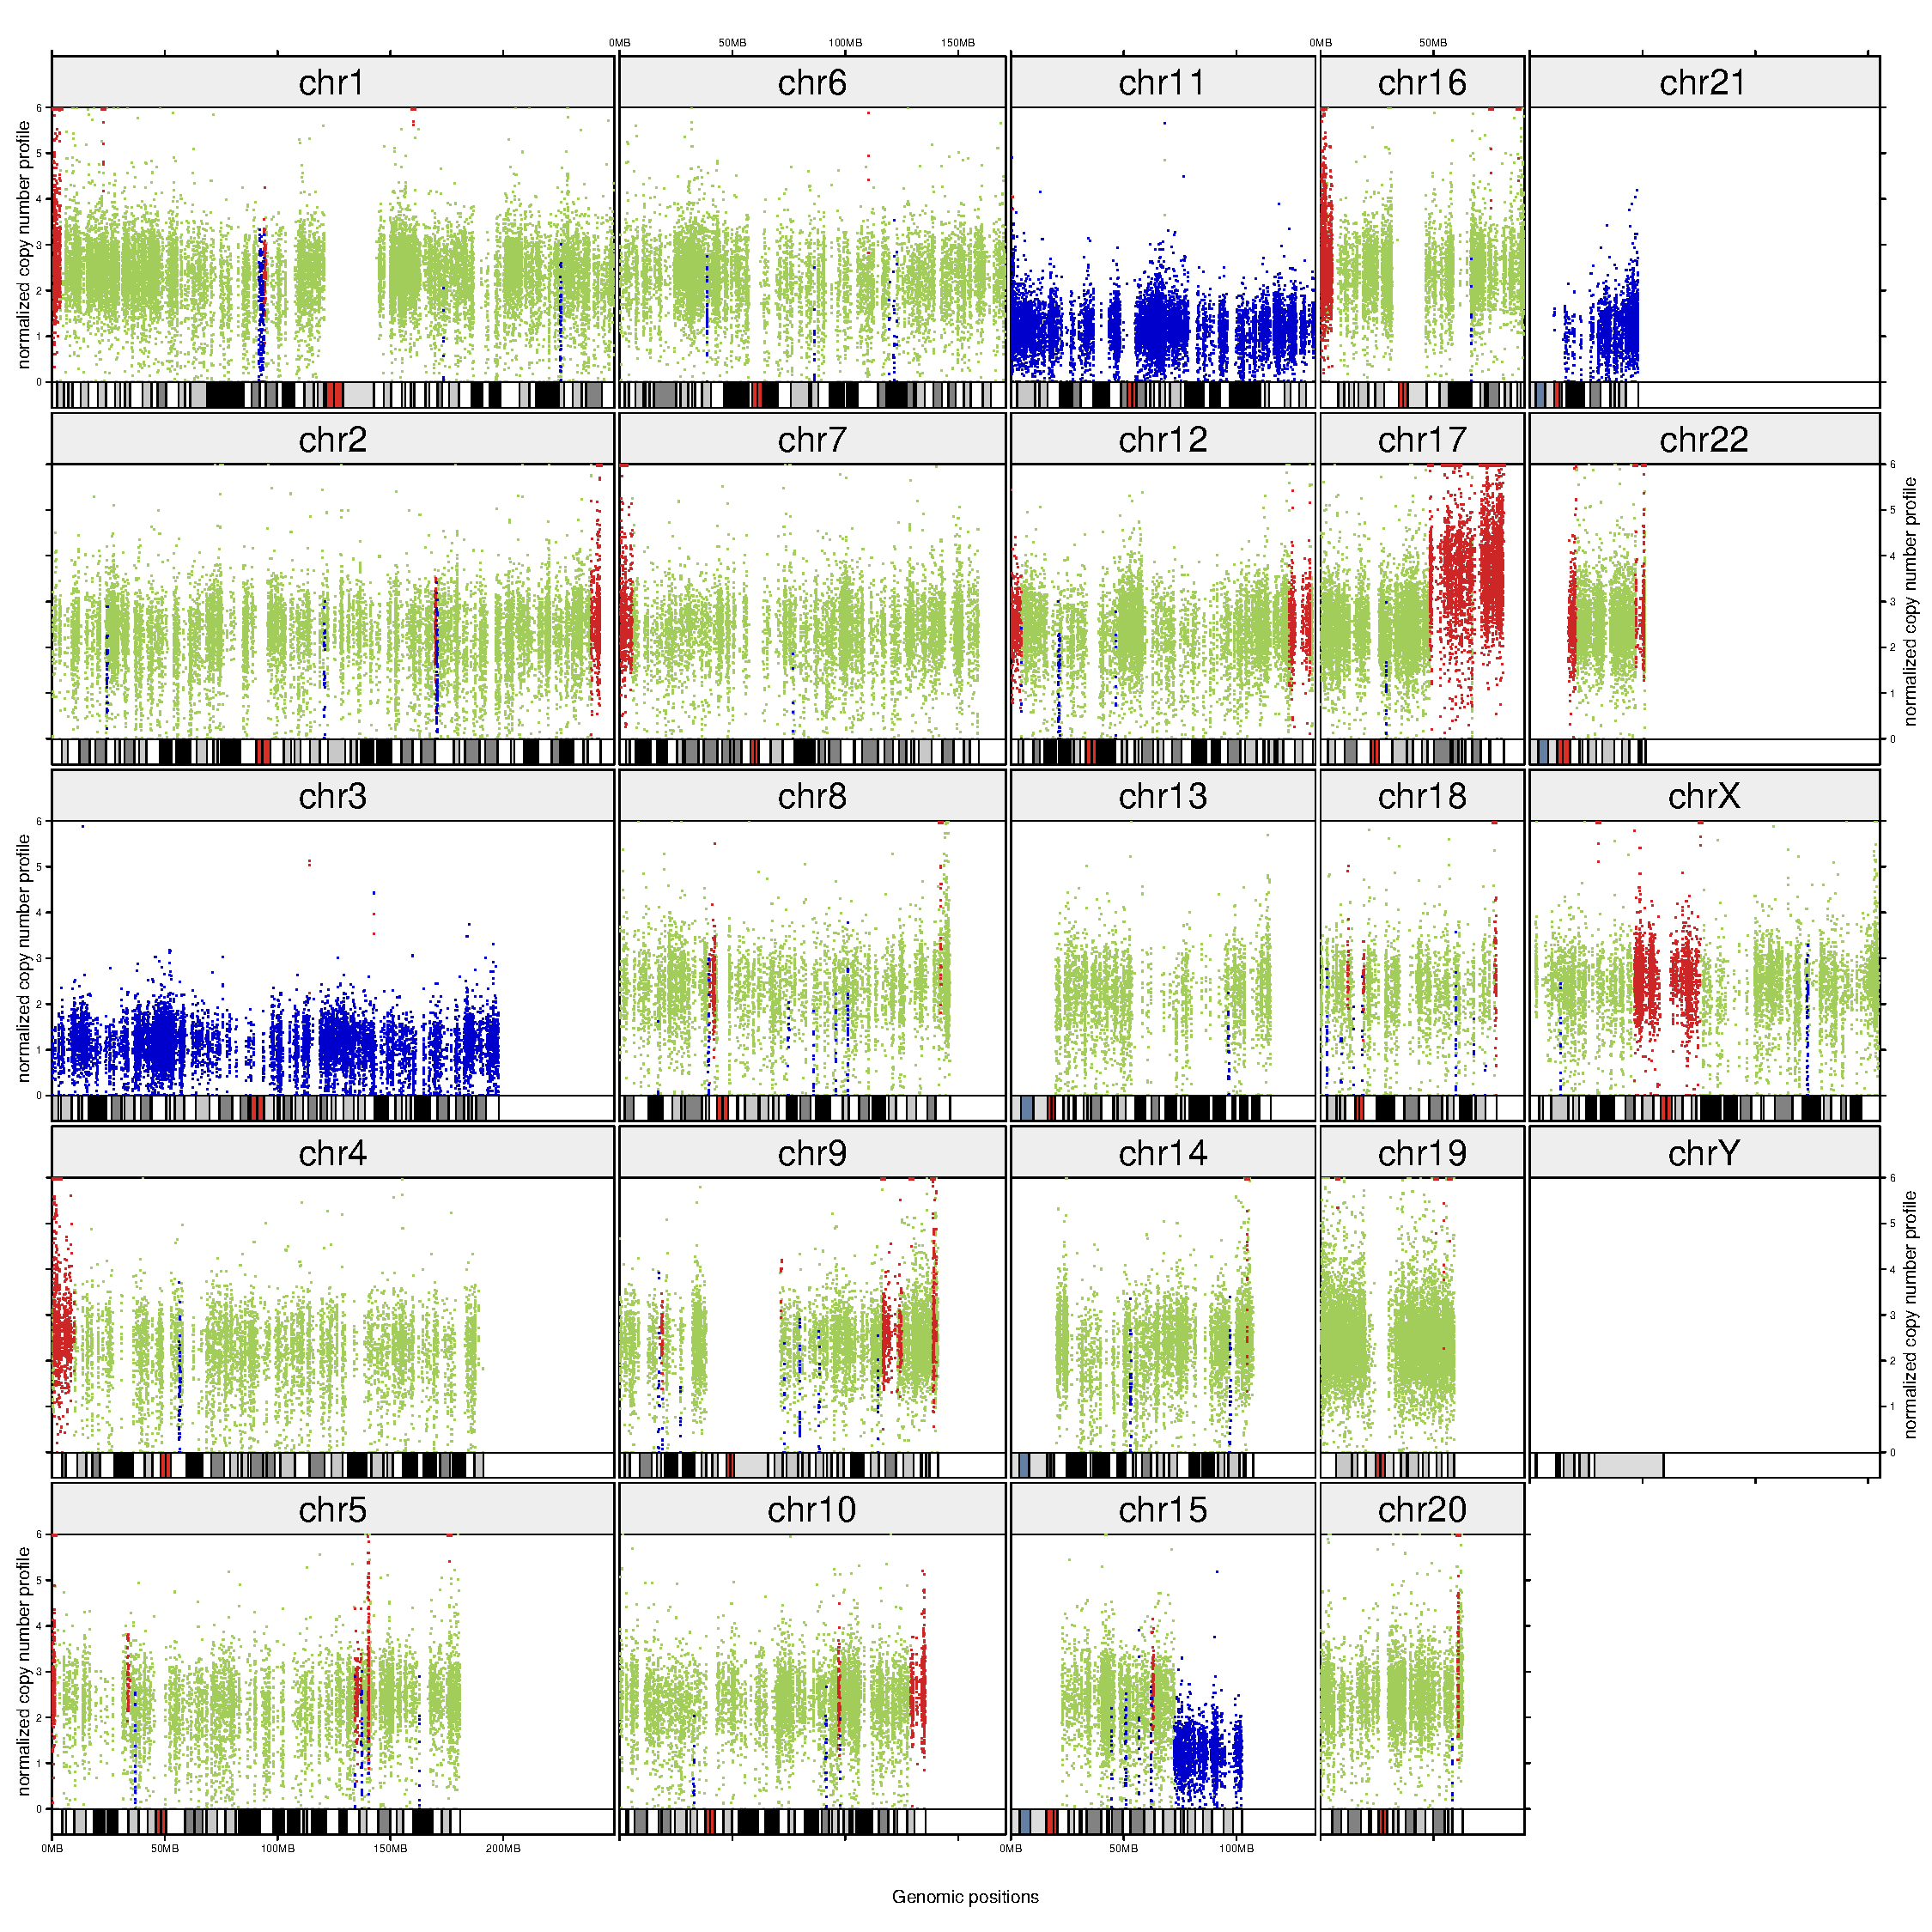
\includegraphics[width=\textwidth]{somaticGermline_TCRBOA6_VCRome_CNV_Plot_2019-02-08.pdf}
\caption{Copy Number Variation}
\label{fig:11}
\end{figure}

\begin{figure}[H]
\centering
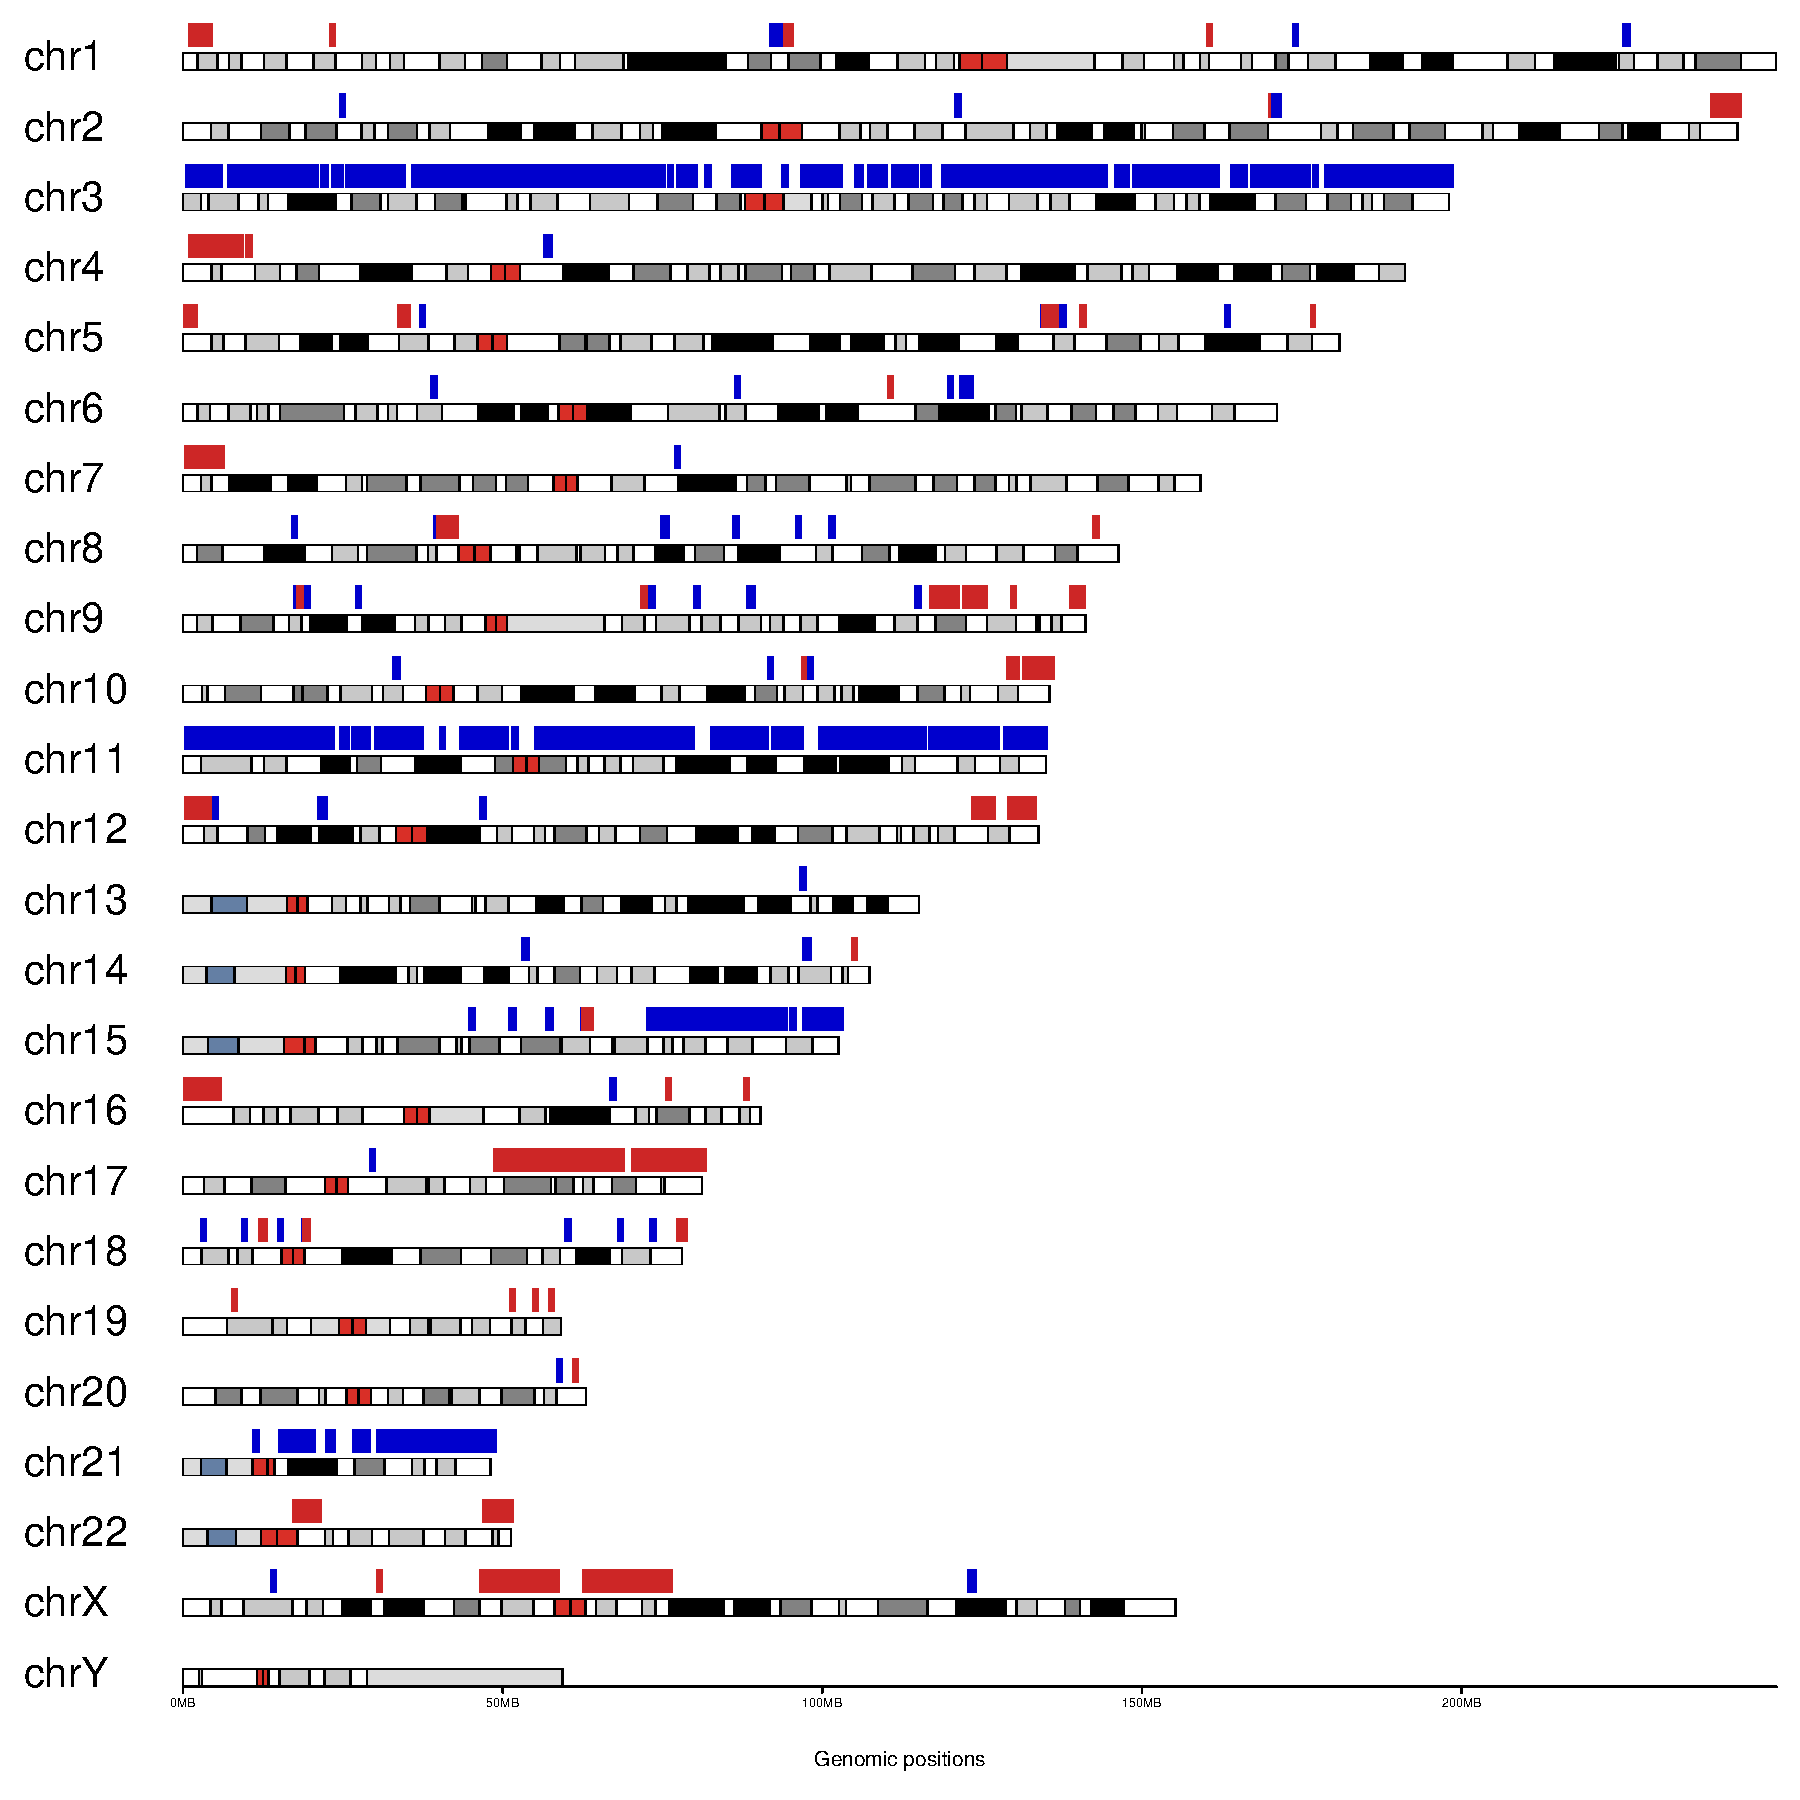
\includegraphics[width=\textwidth]{somaticGermline_TCRBOA6_VCRome_CNV_Plot_Ideogram_2019-02-08.pdf}
\caption{Copy Number Variation - Ideogram}
\label{fig:12}
\end{figure}

\subsection{Tumorsuppressoren}
\begin{knitrout}
\definecolor{shadecolor}{rgb}{0.969, 0.969, 0.969}\color{fgcolor}\rowcolors{2}{gray!6}{white}
\begin{table}[H]

\caption{\label{tab:unnamed-chunk-13}Tumorsuppressoren}
\centering
\begin{tabular}[t]{lrll}
\hiderowcolors
\toprule
chr & copy.number & status & TumorSuppressor\\
\midrule
\showrowcolors
3 & 1 & loss & MLH1,TGFBR2,VHL,BAP1,RYBP,SETD2,SHQ1,PBRM1\\
3 & 1 & loss & ATR\\
5 & 3 & gain & SDHA\\
11 & 1 & loss & MEN1\\
11 & 1 & loss & ATM,CBL,CHEK1,KMT2A,SDHD\\
\addlinespace
15 & 1 & loss & B2M\\
15 & 1 & loss & BLM\\
16 & 3 & gain & TSC2,AXIN1\\
16 & 3 & gain & CREBBP\\
17 & 4 & gain & RAD51C,AXIN2,SPOP,RNF43\\
\addlinespace
21 & 1 & loss & RUNX1\\
X & 3 & gain & RBM10,KDM5C,AMER1\\
\bottomrule
\end{tabular}
\end{table}
\rowcolors{2}{white}{white}


\end{knitrout}

\subsection{Onkogene}
\begin{knitrout}
\definecolor{shadecolor}{rgb}{0.969, 0.969, 0.969}\color{fgcolor}\rowcolors{2}{gray!6}{white}
\begin{table}[H]

\caption{\label{tab:unnamed-chunk-14}Onkogene}
\centering
\begin{tabular}[t]{lrll}
\hiderowcolors
\toprule
chr & copy.number & status & Oncogene\\
\midrule
\showrowcolors
3 & 1 & loss & RHOA,CTNNB1,MYD88,RAF1\\
3 & 1 & loss & PIK3CB\\
3 & 1 & loss & BCL6,PIK3CA,PRKCI\\
4 & 3 & gain & FGFR3\\
5 & 3 & gain & TERT\\
\addlinespace
11 & 1 & loss & HRAS\\
11 & 1 & loss & IGF2\\
11 & 1 & loss & RRAS2\\
11 & 1 & loss & CCND1,FGF3,FGF4,FGF19,YAP1\\
12 & 3 & gain & CCND2\\
\addlinespace
15 & 1 & loss & IDH2,IGF1R,NTRK3\\
17 & 4 & gain & PPM1D\\
17 & 4 & gain & RPTOR\\
21 & 1 & loss & ERG\\
21 & 0 & loss & ERG\\
\addlinespace
21 & 1 & loss & ERG,TMPRSS2,U2AF1\\
X & 3 & gain & AR,ARAF,MED12\\
\bottomrule
\end{tabular}
\end{table}
\rowcolors{2}{white}{white}


\end{knitrout}
\clearpage
\begin{landscape}
\thispagestyle{empty}
\subsection{Funktionelle Analyse der CNVs}
\subsubsection{GAIN}
\begin{knitrout}
\definecolor{shadecolor}{rgb}{0.969, 0.969, 0.969}\color{fgcolor}\rowcolors{2}{white}{gray!6}

\begin{longtable}[t]{>{\raggedright\arraybackslash}p{35em}>{\raggedleft\arraybackslash}p{3em}>{\raggedleft\arraybackslash}p{3em}>{\raggedright\arraybackslash}p{5em}>{\raggedright\arraybackslash}p{3em}}
\caption{\label{tab:unnamed-chunk-15}Ergebnisse GO Analsye - GAIN, top 20}\\
\hiderowcolors
\toprule
Term & Count & Size & p-value & adj.P.Val\\
\midrule
\showrowcolors
embryonic skeletal system development & 11 & 122 & 5.44e-04 & 1e+00\\
negative regulation of mast cell activation & 3 & 12 & 3.76e-03 & 1e+00\\
exploration behavior & 4 & 24 & 3.86e-03 & 1e+00\\
skeletal system morphogenesis & 13 & 209 & 4.49e-03 & 1e+00\\
response to stimulus involved in regulation of muscle adaptation & 3 & 16 & 7.32e-03 & 1e+00\\
\addlinespace
JAK-STAT cascade involved in growth hormone signaling pathway & 3 & 15 & 7.32e-03 & 1e+00\\
endocardial cushion morphogenesis & 4 & 29 & 7.74e-03 & 1e+00\\
embryonic skeletal system morphogenesis & 7 & 93 & 1.41e-02 & 1e+00\\
positive regulation of branching involved in ureteric bud morphogenesis & 3 & 19 & 1.44e-02 & 1e+00\\
regulation of AMPA receptor activity & 3 & 19 & 1.44e-02 & 1e+00\\
\addlinespace
response to growth hormone & 4 & 35 & 1.50e-02 & 1e+00\\
regulation of mast cell activation & 4 & 38 & 1.81e-02 & 1e+00\\
motile cilium assembly & 3 & 23 & 1.89e-02 & 1e+00\\
hydrogen peroxide catabolic process & 3 & 22 & 2.15e-02 & 1e+00\\
growth hormone receptor signaling pathway & 3 & 22 & 2.15e-02 & 1e+00\\
\addlinespace
positive regulation of mesonephros development & 3 & 22 & 2.15e-02 & 1e+00\\
endocardial cushion development & 4 & 39 & 2.16e-02 & 1e+00\\
regulation of long-term neuronal synaptic plasticity & 3 & 23 & 2.42e-02 & 1e+00\\
cartilage development involved in endochondral bone morphogenesis & 3 & 23 & 2.42e-02 & 1e+00\\
cellular response to growth hormone stimulus & 3 & 23 & 2.42e-02 & 1e+00\\
\bottomrule
\end{longtable}
\rowcolors{2}{white}{white}


\end{knitrout}
\clearpage
\subsubsection{LOSS}
\thispagestyle{empty}
\begin{knitrout}
\definecolor{shadecolor}{rgb}{0.969, 0.969, 0.969}\color{fgcolor}\rowcolors{2}{white}{gray!6}

\begin{longtable}[t]{>{\raggedright\arraybackslash}p{35em}>{\raggedleft\arraybackslash}p{3em}>{\raggedleft\arraybackslash}p{3em}>{\raggedright\arraybackslash}p{5em}>{\raggedright\arraybackslash}p{3em}}
\caption{\label{tab:unnamed-chunk-16}Ergebnisse GO Analyse - LOSS, top 20}\\
\hiderowcolors
\toprule
Term & Count & Size & p-value & adj.P.Val\\
\midrule
\showrowcolors
detection of chemical stimulus involved in sensory perception of smell & 174 & 426 & 1.29e-23 & 2.00e-19\\
sensory perception of smell & 182 & 453 & 2.96e-23 & 2.29e-19\\
detection of chemical stimulus involved in sensory perception & 179 & 470 & 2.09e-19 & 1.08e-15\\
detection of stimulus involved in sensory perception & 189 & 520 & 2.90e-17 & 1.12e-13\\
detection of chemical stimulus & 184 & 505 & 4.93e-17 & 1.53e-13\\
\addlinespace
sensory perception of chemical stimulus & 189 & 528 & 1.06e-16 & 2.74e-13\\
detection of stimulus & 215 & 678 & 6.07e-11 & 1.34e-07\\
sensory perception & 263 & 953 & 3.15e-06 & 6.10e-03\\
sodium-independent organic anion transport & 15 & 25 & 4.40e-05 & 7.57e-02\\
urate transport & 8 & 10 & 5.99e-05 & 9.28e-02\\
\addlinespace
adenylate cyclase-inhibiting dopamine receptor signaling pathway & 8 & 11 & 6.94e-04 & 9.78e-01\\
positive regulation of triglyceride catabolic process & 6 & 8 & 2.81e-03 & 1.00e+00\\
behavioral response to cocaine & 10 & 19 & 5.07e-03 & 1.00e+00\\
G-protein coupled purinergic nucleotide receptor signaling pathway & 8 & 14 & 6.39e-03 & 1.00e+00\\
G-protein coupled purinergic receptor signaling pathway & 11 & 23 & 8.35e-03 & 1.00e+00\\
\addlinespace
axon choice point recognition & 5 & 7 & 9.21e-03 & 1.00e+00\\
regulation of triglyceride catabolic process & 7 & 12 & 9.32e-03 & 1.00e+00\\
negative regulation of cyclase activity & 13 & 30 & 1.16e-02 & 1.00e+00\\
axon midline choice point recognition & 4 & 5 & 1.18e-02 & 1.00e+00\\
regulation of basement membrane assembly involved in embryonic body morphogenesis & 4 & 5 & 1.18e-02 & 1.00e+00\\
\bottomrule
\end{longtable}
\rowcolors{2}{white}{white}


\end{knitrout}
\clearpage
\end{landscape}

\section{Analyse der Mutationssignaturen}

\begin{itemize}
\item Nur somatische Mutationen werden berücksichtigt
\item Nur Signaturen, die mehr als $1\%$ aller SNVs beinhalten, werden verwendet
\item Die Signautren basieren auf den aktuellen \textit{COSMIC Mutation Signatures} \url{http://cancer.sanger.ac.uk/cosmic/signatures}
\item \textit{AC3} wird als \textit{BRCAness} bezeichnet
\end{itemize}

\begin{knitrout}
\definecolor{shadecolor}{rgb}{0.969, 0.969, 0.969}\color{fgcolor}\rowcolors{2}{gray!6}{white}
\begin{table}[H]

\caption{\label{tab:unnamed-chunk-17}Ergebnisse Mutationssignatur Analyse}
\centering
\begin{tabular}[t]{llr}
\hiderowcolors
\toprule
Signature & Process & Percentage\\
\midrule
\showrowcolors
AC2 & APOBEC & 3.46\\
AC3 & defect DNA DSB repair hom. recomb. & 18.04\\
AC12 & unknown & 11.04\\
AC13 & APOBEC & 1.50\\
AC15 & defect DNA MMR & 6.80\\
\addlinespace
AC20 & associated w. small indels at repeats & 31.87\\
AC21 & unknown & 2.01\\
AC22 & aristocholic acid & 3.94\\
AC23 & unknown & 2.22\\
AC29 & tobacco chewing & 6.10\\
AC30 & unknown & 13.02\\
\bottomrule
\end{tabular}
\end{table}
\rowcolors{2}{white}{white}


\end{knitrout}

\clearpage

\section{Versionsinfo}

\subsection{Genome}
\begin{itemize}
\item UCSC hg19
\end{itemize}

\subsection{Programmversionen}
\begin{itemize}
\item FastQC: 0.11.5
\item Trimmomatic: 0.38
\item BWA: 0.7.17
\item bam-readcount: 0.8.0
\item samtools 1.9
\item GATK: 3.8.1.0
\item picard-tools: 2.18.15
\item VarScan: 2.4.3
\item annovar 2018-04-16
\item bedtools: 2.27.1
\item Control-FREEC: 11.0
\item Java: 1.8.0\_152
\item R: 3.4.1
\end{itemize}

\subsection{Annovar Datenbanken}
\begin{itemize}
\item refGene GRCh37
\item esp6500siv2\_ea (ESP3500, European)
\item avsnp150 (dbSNP)
\item EU.sites.2015\_08 (1000Genome, European)
\item cosmic86
\item exac03 (ExAC)
\item gnomad\_exome
\item clinvar\_20180603
\item intervar\_20180118
\item dbnsfp35a
\item cadd13
\end{itemize}

\end{document}
